%!TEX root = ../thesis.tex
\chapter{Closening MAS Simulation and Development through a JADE-based API}
\label{chap:solution}

The modelling of MAS can be accomplished through the use of a wide range of available platforms, as explained before. In certain cases, in order to benefit from different features, modelling the same system in multiple development environments may be necessary.

As explained in Introduction, the two mains goals of this thesis are the creation of an adapter to provide abstraction from MABS frameworks, allowing the creation of JADE-based simulations, and the creating of a mechanism that uses this adapter to convert MABS into MAS. To accomplish these goals, an integrated system was designed, which comprises two main components :

\begin{enumerate}
  \item The \textbf{Simple API for JADE-based Simulations (SAJaS)}, which provides a set of features present in JADE; those features were reimplemented from scratch in an attempt to simplify their internal complexity, preserving JADE-like external execution;
  \item The \textbf{Code Conversion Tool} in the form of an Eclipse plug-in that is capable of mapping JADE and SAJaS features and convert applications developed using one into applications based on the other, automatically. The plugin has no Repast or JADE dependencies in the code, buts contains a dictionary file that is specific to JADE and Repast.
\end{enumerate}

This chapter makes a high level overview of both components and how they work together. After an overview in the next section, Section \ref{sec:solution-fipa} explains how FIPA standards for agent interaction and management are implemented in SAJaS. Section \ref{sec:solution-scenarios} contains a description of the expected scenarios where this system could be used.

\section{Overview}
\label{sec:solution-overview}
%In this section, explain the integrated solution of SAJaS + plug-in, how they work, what they use in terms of dependencies, etc.

SAJaS is an API meant to be used with simulation frameworks to enable JADE-based features in them, including agent interaction protocols and agent management services. The API also uses JADE's concept of behaviours which encapsulate most of agents' actions.

SAJaS was initially created to be used with Repast Simphony. However, it was developed in a way that allows its integration with other simulation tools. The interface between Repast and SAJaS is made in a single point, the Scheduler, which is a Repast-specific structure. If developers desire to add support for other simulation frameworks, different implementations of the scheduler can be created.

Another important aspect kept in mind when developing SAJaS was the importance of keeping a close semblance to JADE's own API not only to make the code  conversion more straightforward, but to allow proficient JADE developers to crete SAJaS-based simulations using familiar JADE tools. The code conversion tool was developed as an Eclipse plugin. It provides programmers with two possible actions: convert code from JADE to SAJaS and in the opposite direction.

SAJaS does not yet implement all JADE features. For the purposes of this thesis, a set of the most common features were selected which allows for the simulation of scenarios with some complexity, including negotiation between agents and the creation of custom behaviours. Features in JADE applications which are not available in SAJaS will typically be shown as errors when converted; the plugin simply ignores them and they should be re-implemented manually as necessary. Chapter \ref{chap:validation} shows examples of scenarios created with SAJaS and JADE that were successfully converted while preserving functionality.

Figure \ref{fig:related-repacl} tries to compare \apiname{} with JRep and MISIA, described in Chapter \ref{chap:background}. The API's general structure is simpler; it does not intend to maintain an active connection to a JADE platform, eliminating the need for synchronization. Instead, our goal is to replicate in our API the main features of JADE, allowing for a straightforward and dependency free feature mapping between our API and JADE.

\begin{figure}
	\centering
	\includegraphics[width=0.5\linewidth]{figures/repacl.pdf}
	\caption{Basic structure of \apiname{}}
	\label{fig:related-repacl}
\end{figure}

\section{FIPA Specifications}
\label{sec:solution-fipa}

Part of the rationale for the creation of SAJaS was to enable agent interaction standards in otherwise standard-less simulation frameworks, namely Repast, the one featured in this thesis. This section explains the FIPA standards for agent interaction and management implemented in SAJaS.

As mentioned before, SAJaS follows JADE architecture very closely, including how FIPA standards are implemented. The implemented features can be divided in the following categories:

\begin{enumerate}
  \item \textbf{Agent Management}, which includes the directory facilitator (DF) service, the structures used by it and the Agent Management Service (AMS),
  \item \textbf{Messaging}, including the ACL Message, the Message Template and the Message Transport Service (MTS), and
  \item \textbf{Interaction Protocols} that allow agents to exchange ACL Messages in a standardized manner.
\end{enumerate}

\subsection{Agent Management}
The AMS functions as a directory of all agents in a MAS and every agent is automatically registered in the AMS upon its initialization. BY the time they are registered, agents are also assigned an Agent Identifier (AID) used throughout the application. Only the AMS and the agent itself know who the AID belongs to.

The DF is a facultative directory where agents can register themselves as service providers. The DF Agent Description is a structure used to describe one agent when it registers itself in the DF or to describe a group of agents when performing a search. The DF Agent Description can contain one or more Service Descriptions. The fields of these structures are listed in table \ref{tab:dfAgentDescription}.

\begin{table}
	\normalsize
	\caption[The DF Agent Descriptions and the Service Description]{Information contained in the DF Agent Descriptions and Service Description structures.
	M: Mandatory field. S: Mandatory when agent registers.}
	\label{tab:dfAgentDescription}
	\begin{center}
		\begin{tabular}{c|c}
		\hline
		\textbf{DFAgentDescription} & \textbf{ServiceDescription} \\
		\hline
		name \textsuperscript{S} : AID & service name \textsuperscript{M} : String \\
		\hline
		services : ServiceDescriptions & type \textsuperscript{M} : String \\
		\hline
		\multicolumn{2}{c}{protocols : Strings} \\
		\hline
		\multicolumn{2}{c}{ontologies : Strings} \\
		\hline
		\multicolumn{2}{c}{languages : Strings} \\
		\hline
		\end{tabular}
	\end{center}
\end{table} 

\subsection{Messaging}
The implementation of the ACL Message is essentially identical to JADE's. SAJaS also implements the Message Template, which is used to filter incoming messages. A series of template factories exist in the API that allow one to create message templates. 

\subsection{Interaction Protocols}
% The interaction protocols in the api
JADE has the support for many interaction protocols. The most common ones were selected to be included in \apiname{}.
% The specific protocols
The implemented protocols were the ``request-like'' Achieve Rational Effect (AchieveRE) protocol, the Contract Net protocol and the Single Session Contract Net - including the Responder Dispatcher behaviour, which uses it.

The AchieveRE encompasses multiple \gls{FIPA} protocols, namely Request, Query, Request-When, Recruiting and Brokering protocols, as defined in JADE's documentation.

\section{Usage Scenarios}
\label{sec:solution-scenarios}
%In this section, show how the whole setup is used with detailed use cases
This section is meant to describe both the scenarios where this system is expected to be useful, as well as the actual possible use cases. Figure \ref{fig:prototypeFlow} illustrates these scenarios.

One possible scenario is when a JADE developer created a JADE MAS and desires to perform some tests and simulations in a local and controlled environment. The developer can use this tool to convert the MAS into a MABS. Eventually, the application can be converted back if changes were made while in the simulation format.

A second possible scenario could be that of a developer that intends to create a MABS with the goal of later creating a MAS out of it. This could be a Repast developer who desires to create more complex agent simulations or a JADE developer that wants to create Repast simulations using familiar JADE-like tools.

A third scenario is when a developer simply wants to create a complex agent-based, FIPA-compliant simulation. In this case, there is no need for a code conversion tool, but SAJaS can be used as a standalone library.

\begin{figure}
	\centering
	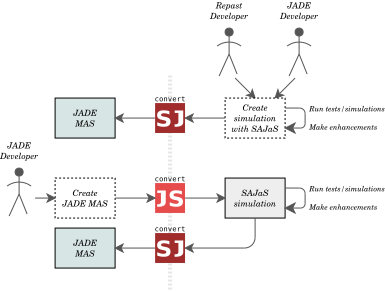
\includegraphics[width=0.9\linewidth]{figures/prototypeFlow.pdf}
	\caption{
		Two possible workflows for \apiname{} users
	}
	\label{fig:prototypeFlow}
\end{figure}

